%!TEX root = ../main.tex
\chapter{Krav}
Ud fra opgaveformuleringen er der udarbejdet en række \gls{usecase}s, som beskriver aktørernes interaktion med systemet. Disse \gls{usecase}s er anvendt i kravspecifikationen, og er brugt som udgangspunkt til at fastlægge systemets funktionalitet og handlingsforløb med omverdenen. De fulde \gls{usecase}s kan findes i kravspecifikationen i dokumentationen, sammen med de ikke-fully dressed \gls{usecase}s og de funktionelle krav.
\newline

\begin{minipage}{0.45\textwidth}
\raggedright
\section{Aktørbeskrivelse}
I \gls{usecase}ne ses en række aktører, der interagerer med systemet. Disse kan ses på aktørdiagrammet i figur~\ref{fig:actordiagram} og er beskrevet herunder. Flere detaljer om aktørerne og hvordan de interagerer med de ikke fully-dressed \gls{usecase}s kan ses i dokumentationen. 
\newline
\newline
\end{minipage}
\begin{minipage}{0.55\textwidth}
\begin{figure}[H]
	\centering
	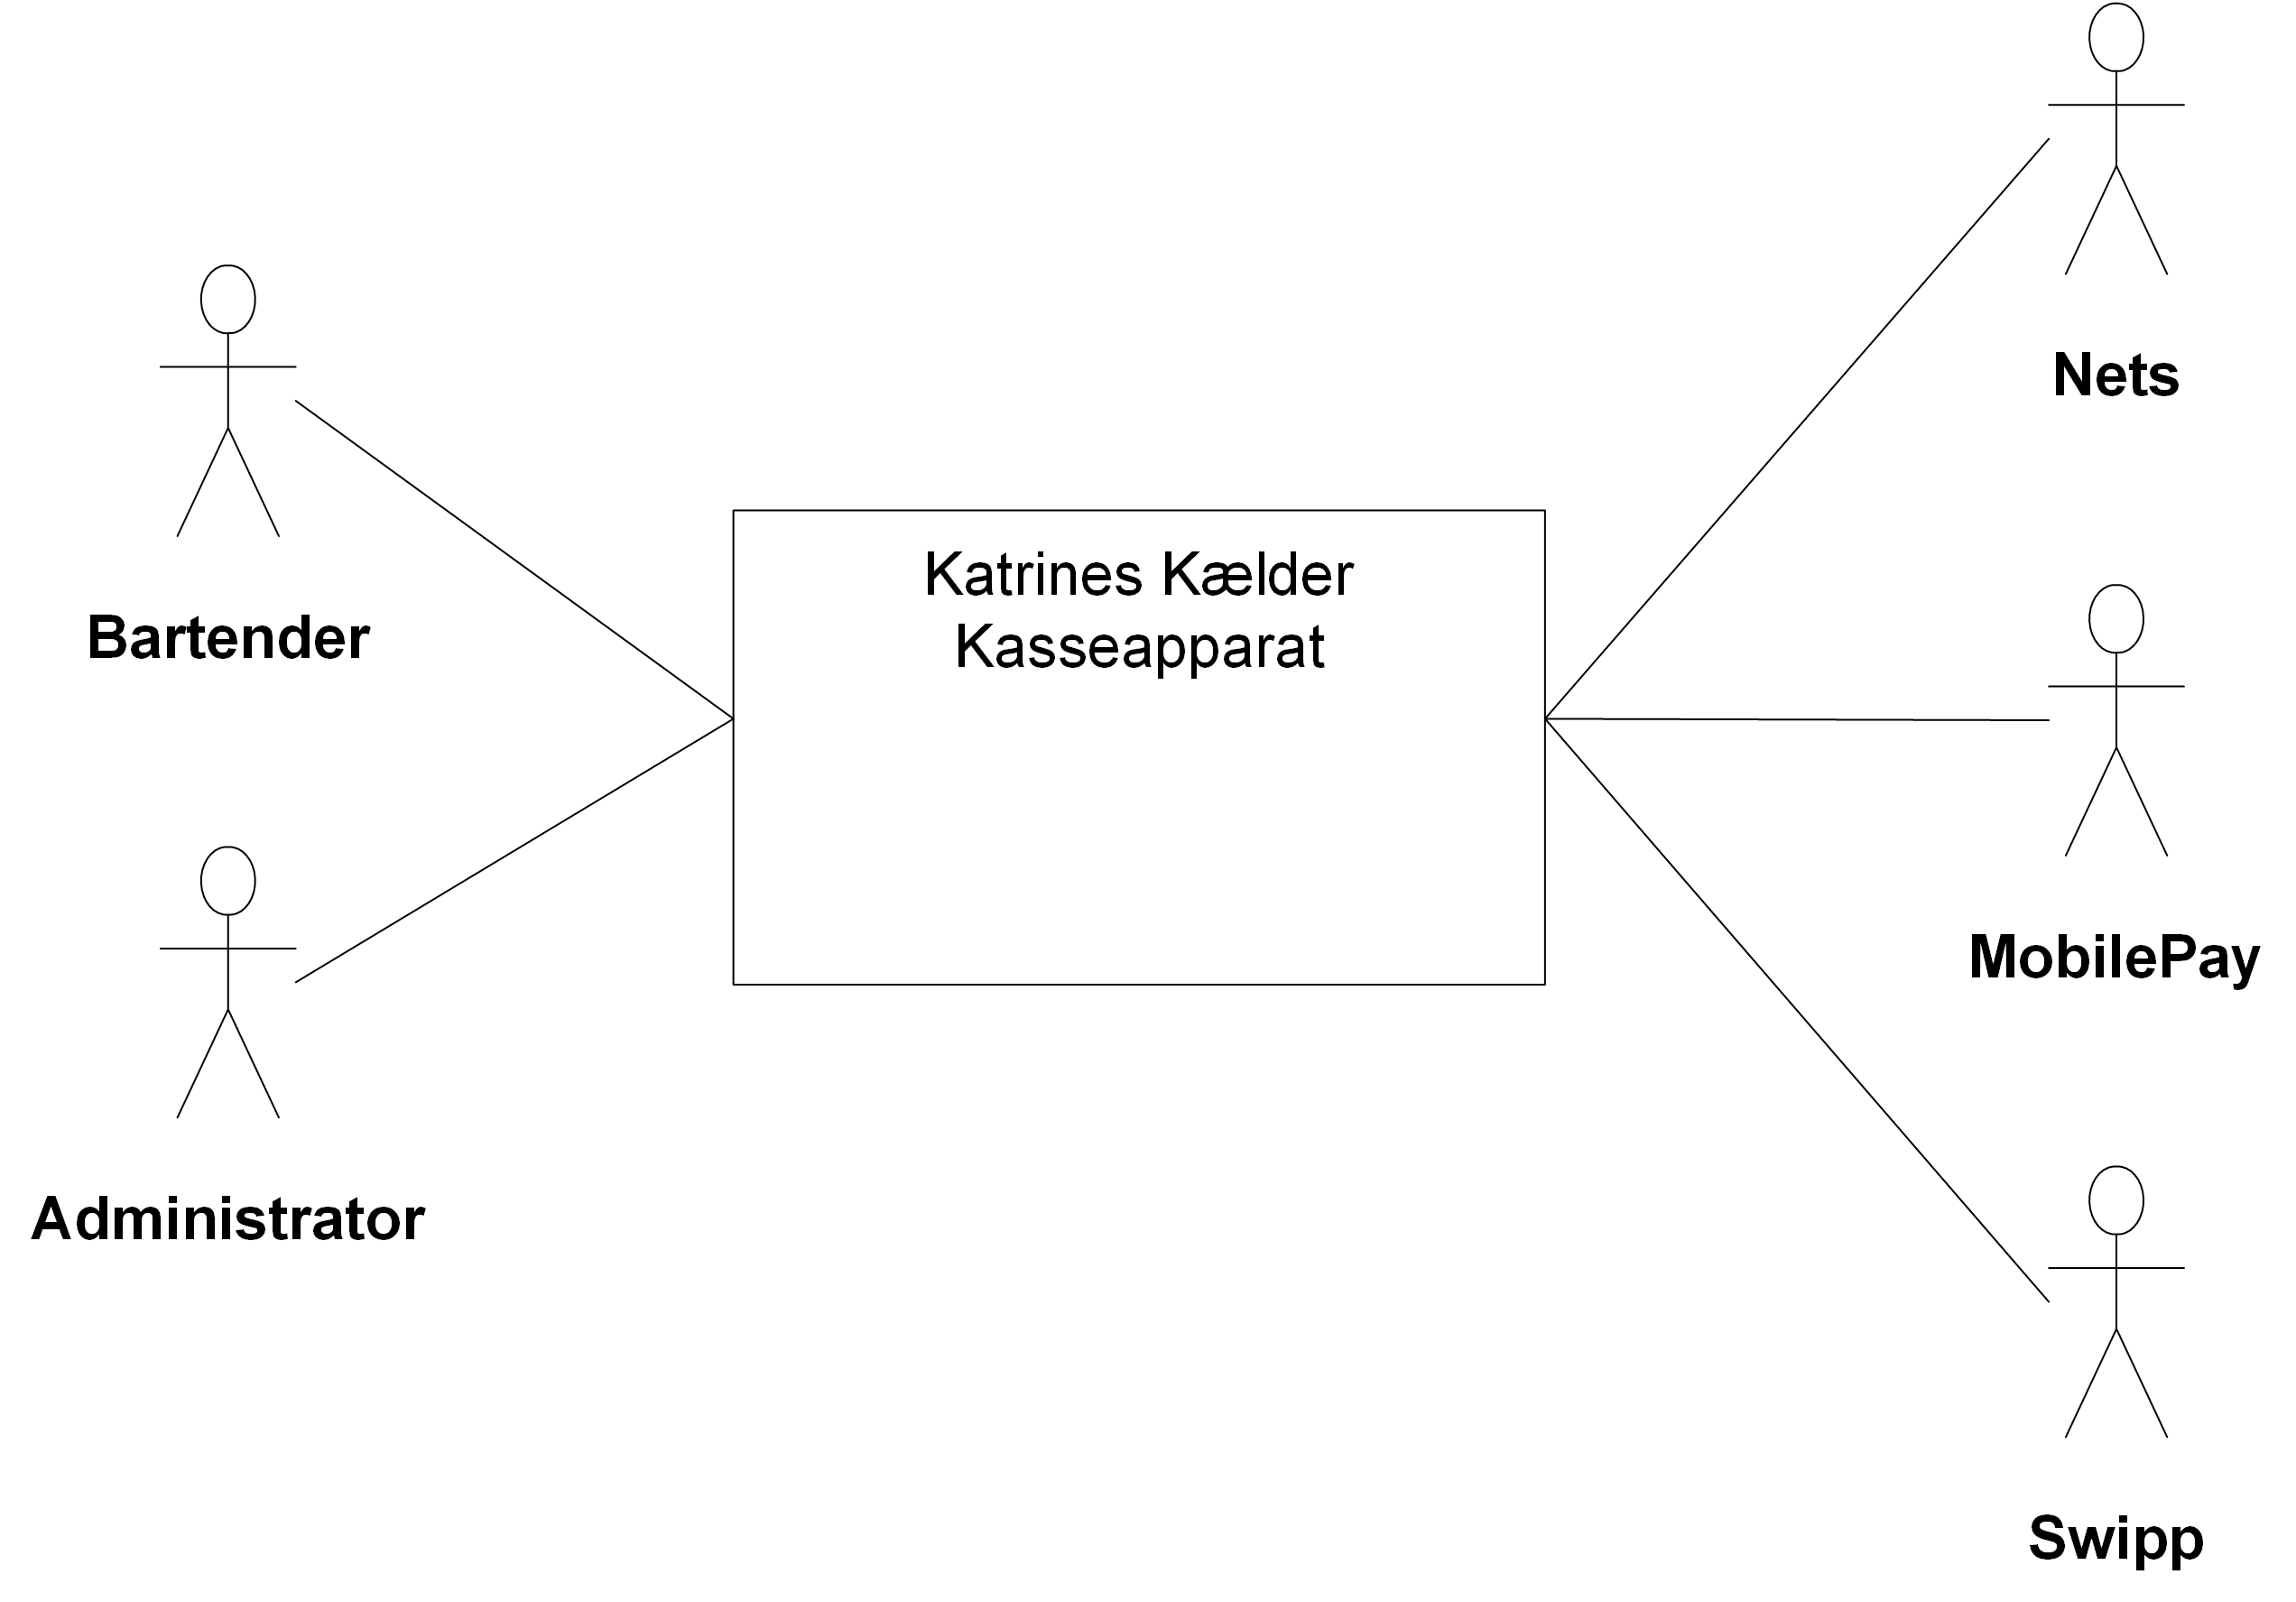
\includegraphics[width=0.7\textwidth]{Kravspecifikation/Actor/Actor.png}
	\caption{Aktør-kontekst diagram}
	\label{fig:actordiagram}
\end{figure}
\end{minipage} \hfill
\newline
\subsubsection*{\Gls{bartender}}
er en primær aktør til systemet, og står for salg af varer og betjening. 

\subsubsection*{\Gls{administrator}}
er en primær aktør til systemet, som står for logistikken (priser, varer osv.). 

\subsubsection*{Nets}
er en sekundær aktør, som er leverandøren af den \gls{betalingsterminal}, hvor der kan bruges \gls{betalingskort}. Dette er en af systemets primære betalingsløsning.

\subsubsection*{MobilePay} 
er en sekundær aktør, det er en betalingsløsning via mobiltelefonen, som er leveret af Danske Bank.

\subsubsection*{Swipp} 
er en sekundær aktør, som er en betalingsløsning via mobiltelefonen som leveres af Nordea, Nykredit, Sydbank, Jyske Bank, Arbejdernes Landsbank, Spar Nord Bank og Lokale Pengeinstitutter.

\newpage

\section{Use case beskrivelse}
De identificerede \gls{usecase}s er beskrevet i det følgende. Her er der kun fokus på de fully-dressed \gls{usecase}s. Hver \gls{usecase} beskriver et scenarie, hvor aktører interagerer med systemet. I Figur~\ref{fig:fullydressedusecases} kan der ses et \gls{usecase} diagram med hvilke aktører som er involverede.

\begin{figure}[H]
	\centering
	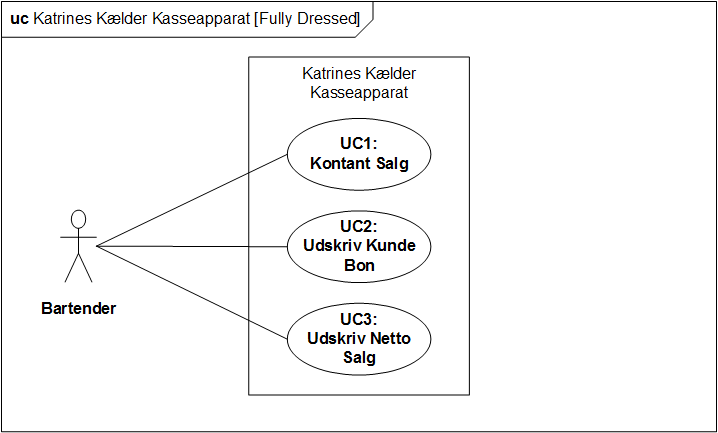
\includegraphics[width=0.45\textwidth]{Kravspecifikation/UseCases/UseCases_fully_dressed.png}
	\caption{\gls{usecase} diagram for de fully dressed \gls{usecase}.}
	\label{fig:fullydressedusecases}
\end{figure} 

\subsection*{Use Case 1: Kontant salg}
Bartenderen skal kunne sælge varer mod kontant betaling. Det sker ved, at bartenderen trykker på de varer, som kunden ønsker. Når ordren er slut, vælger \gls{bartender} kontant betaling i betalingsvinduet.

\subsection*{Use Case 2: Udskriv kundebon}
Hvis en kunde ønsker en bon, skal en \gls{bartender} kunne printe den ud. Dette bliver gjort ved at trykke på bon knappen, som udskriver en bon via bonprinteren.

\subsection*{\gls{usecase} 3: Kasseafstemning}
Når der skal printes en bon, med hvor meget der er solgt for i løbet af en salgsdag, trykker bartenderen på afstem knappen og bonprinteren printer en bon med dato og det samlede salg. 

\subsection*{\gls{usecase} 9: Tilføj vare til kasseapparat}
Det skal være muligt at tilføje flere varer til kasseapparatet. Dette kan \gls{administrator} gøre ved at gå ind under settings i \gls{WebAPI}'en og tilføje et produkt ved at udfylde felterne i \textit{Add Product} og trykke \textit{Submit}.

\subsection*{\gls{usecase} 10: Rediger vare i kasseapparat}
En vare skal kunne redigeres, hvis der f.eks. skal nye priser på. Dette gør \gls{administrator} ved at vælge den vare som han ønsker at redigere. Dette gøres under \textit{Settings} i \gls{WebAPI}. Her kan de ønskede værdier ændres og gemmes ved at trykke \textit{Submit}.

\subsection*{\gls{usecase} 11: Fjern vare fra kasseapparat}
En vare skal kunne fjernes. Det gør \gls{administrator} ved at vælge den vare som han ønsker slettet under \textit{Settings} i \gls{WebAPI} og trykke på \textit{Delete} ud for varen.